% This file was created with tikzplotlib v0.10.1.
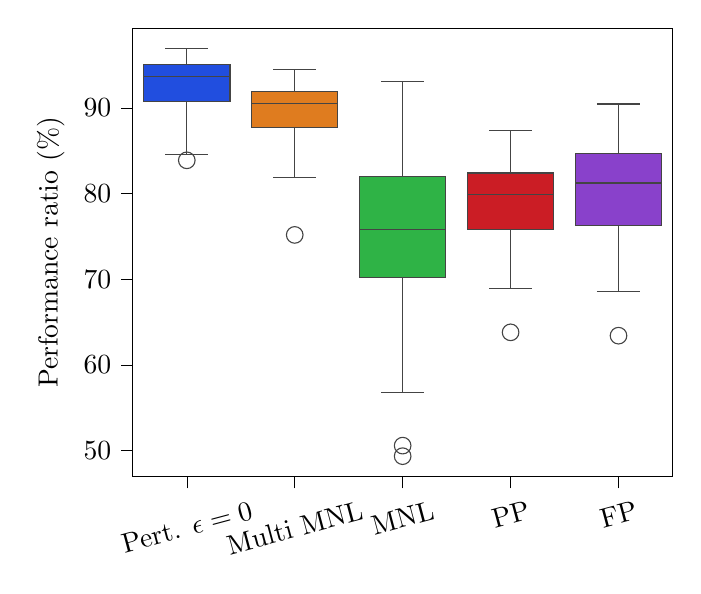
\begin{tikzpicture}

\definecolor{chocolate22312431}{RGB}{223,124,31}
\definecolor{darkgray176}{RGB}{176,176,176}
\definecolor{darkorchid13765203}{RGB}{137,65,203}
\definecolor{darkslategray68}{RGB}{68,68,68}
\definecolor{firebrick2032937}{RGB}{203,29,37}
\definecolor{limegreen4717970}{RGB}{47,179,70}
\definecolor{royalblue3378223}{RGB}{33,78,223}

\begin{axis}[
tick align=outside,
tick pos=left,
x grid style={darkgray176},
xmin=-0.5, xmax=4.5,
xtick style={color=black},
xtick={0,1,2,3,4},
xticklabel style={rotate=15.0},
xticklabels={Pert. \(\displaystyle \epsilon=0\),Multi MNL,MNL,PP,FP},
y grid style={darkgray176},
ylabel={Performance ratio (\%)},
ymin=46.9641574196683, ymax=99.3026105344177,
ytick style={color=black},
ytick={40,50,60,70,80,90,100},
yticklabels={
  \(\displaystyle {40}\),
  \(\displaystyle {50}\),
  \(\displaystyle {60}\),
  \(\displaystyle {70}\),
  \(\displaystyle {80}\),
  \(\displaystyle {90}\),
  \(\displaystyle {100}\)
}
]
\path [draw=darkslategray68, fill=royalblue3378223]
(axis cs:-0.4,90.7945482505667)
--(axis cs:0.4,90.7945482505667)
--(axis cs:0.4,95.0250109392938)
--(axis cs:-0.4,95.0250109392938)
--(axis cs:-0.4,90.7945482505667)
--cycle;
\addplot [darkslategray68]
table {%
0 90.7945482505667
0 84.605982889528
};
\addplot [darkslategray68]
table {%
0 95.0250109392938
0 96.9235899382927
};
\addplot [darkslategray68]
table {%
-0.2 84.605982889528
0.2 84.605982889528
};
\addplot [darkslategray68]
table {%
-0.2 96.9235899382927
0.2 96.9235899382927
};
\addplot [black, mark=o, mark size=3, mark options={solid,fill opacity=0,draw=darkslategray68}, only marks]
table {%
0 83.8823287736362
};
\path [draw=darkslategray68, fill=chocolate22312431]
(axis cs:0.6,87.7259901591438)
--(axis cs:1.4,87.7259901591438)
--(axis cs:1.4,91.8675688551704)
--(axis cs:0.6,91.8675688551704)
--(axis cs:0.6,87.7259901591438)
--cycle;
\addplot [darkslategray68]
table {%
1 87.7259901591438
1 81.8339690381899
};
\addplot [darkslategray68]
table {%
1 91.8675688551704
1 94.4436556843885
};
\addplot [darkslategray68]
table {%
0.8 81.8339690381899
1.2 81.8339690381899
};
\addplot [darkslategray68]
table {%
0.8 94.4436556843885
1.2 94.4436556843885
};
\addplot [black, mark=o, mark size=3, mark options={solid,fill opacity=0,draw=darkslategray68}, only marks]
table {%
1 75.1728426862789
};
\path [draw=darkslategray68, fill=limegreen4717970]
(axis cs:1.6,70.1600619168688)
--(axis cs:2.4,70.1600619168688)
--(axis cs:2.4,81.9879878856474)
--(axis cs:1.6,81.9879878856474)
--(axis cs:1.6,70.1600619168688)
--cycle;
\addplot [darkslategray68]
table {%
2 70.1600619168688
2 56.7600264906113
};
\addplot [darkslategray68]
table {%
2 81.9879878856474
2 93.0645193576326
};
\addplot [darkslategray68]
table {%
1.8 56.7600264906113
2.2 56.7600264906113
};
\addplot [darkslategray68]
table {%
1.8 93.0645193576326
2.2 93.0645193576326
};
\addplot [black, mark=o, mark size=3, mark options={solid,fill opacity=0,draw=darkslategray68}, only marks]
table {%
2 49.3431780157933
2 50.5735419693593
};
\path [draw=darkslategray68, fill=firebrick2032937]
(axis cs:2.6,75.8449688825698)
--(axis cs:3.4,75.8449688825698)
--(axis cs:3.4,82.4022993199884)
--(axis cs:2.6,82.4022993199884)
--(axis cs:2.6,75.8449688825698)
--cycle;
\addplot [darkslategray68]
table {%
3 75.8449688825698
3 68.8724611986297
};
\addplot [darkslategray68]
table {%
3 82.4022993199884
3 87.3404238482497
};
\addplot [darkslategray68]
table {%
2.8 68.8724611986297
3.2 68.8724611986297
};
\addplot [darkslategray68]
table {%
2.8 87.3404238482497
3.2 87.3404238482497
};
\addplot [black, mark=o, mark size=3, mark options={solid,fill opacity=0,draw=darkslategray68}, only marks]
table {%
3 63.8000644930302
};
\path [draw=darkslategray68, fill=darkorchid13765203]
(axis cs:3.6,76.2521834388413)
--(axis cs:4.4,76.2521834388413)
--(axis cs:4.4,84.6809458763638)
--(axis cs:3.6,84.6809458763638)
--(axis cs:3.6,76.2521834388413)
--cycle;
\addplot [darkslategray68]
table {%
4 76.2521834388413
4 68.6061398541417
};
\addplot [darkslategray68]
table {%
4 84.6809458763638
4 90.4525199239857
};
\addplot [darkslategray68]
table {%
3.8 68.6061398541417
4.2 68.6061398541417
};
\addplot [darkslategray68]
table {%
3.8 90.4525199239857
4.2 90.4525199239857
};
\addplot [black, mark=o, mark size=3, mark options={solid,fill opacity=0,draw=darkslategray68}, only marks]
table {%
4 63.4092235156811
};
\addplot [darkslategray68]
table {%
-0.4 93.6450521490036
0.4 93.6450521490036
};
\addplot [darkslategray68]
table {%
0.6 90.486263555085
1.4 90.486263555085
};
\addplot [darkslategray68]
table {%
1.6 75.777345484792
2.4 75.777345484792
};
\addplot [darkslategray68]
table {%
2.6 79.9065168022921
3.4 79.9065168022921
};
\addplot [darkslategray68]
table {%
3.6 81.2345523599997
4.4 81.2345523599997
};
\draw (axis cs:0,33.879544140981) node[
  scale=0.75,
  anchor=base,
  text=black,
  rotate=0.0
]{\bfseries 92.63};
\draw (axis cs:1,33.879544140981) node[
  scale=0.75,
  anchor=base,
  text=black,
  rotate=0.0
]{\bfseries 89.57};
\draw (axis cs:2,33.879544140981) node[
  scale=0.75,
  anchor=base,
  text=black,
  rotate=0.0
]{\bfseries 75.53};
\draw (axis cs:3,33.879544140981) node[
  scale=0.75,
  anchor=base,
  text=black,
  rotate=0.0
]{\bfseries 79.24};
\draw (axis cs:4,33.879544140981) node[
  scale=0.75,
  anchor=base,
  text=black,
  rotate=0.0
]{\bfseries 80.48};
\draw (axis cs:-1,34.4029286721285) node[
  scale=0.75,
  text=black,
  rotate=0.0
]{\bfseries \textbf{Average:}};
\end{axis}

\end{tikzpicture}
